\documentclass[twocolumn,a4j]{jsarticle}
\setlength{\topmargin}{-20.4cm}
\setlength{\oddsidemargin}{-10.4mm}
\setlength{\evensidemargin}{-10.4mm}
\setlength{\textwidth}{18cm}
\setlength{\textheight}{26cm}

\usepackage[top=15truemm,bottom=20truemm,left=20truemm,right=20truemm]{geometry}
\usepackage[latin1]{inputenc}
\usepackage{amsmath}
\usepackage{amsfonts}
\usepackage{amssymb}
\usepackage[dvipdfmx]{graphicx}
\usepackage[hang,small,bf]{caption}
\usepackage[subrefformat=parens]{subcaption}
\usepackage[dvipdfmx]{color}
\usepackage{listings}
\usepackage{listings,jvlisting}
\usepackage{geometry}
\usepackage{framed}
\usepackage[dvipdfmx]{hyperref}
\usepackage{ascmac}
\usepackage{enumerate}
\usepackage{tabularx}
\usepackage{cancel}
\usepackage{scalefnt}
\usepackage{overcite}
\usepackage{otf}
\usepackage{multicol}
\usepackage[geometry]{ifsym}
\usepackage{array}

\renewcommand{\figurename}{Fig.}
\renewcommand{\tablename}{Table }

\lstset{
basicstyle={\ttfamily},
identifierstyle={\small},
commentstyle={\smallitshape},
keywordstyle={\small\bfseries},
ndkeywordstyle={\small},
stringstyle={\small\ttfamily},
frame={tb},
breaklines=true,
columns=[l]{fullflexible},
xrightmargin=0zw,
xleftmargin=3zw,
numberstyle={\scriptsize},
stepnumber=1,
numbersep=1zw,
lineskip=-0.5ex
}

% キャプション後ろのダブルコロンを消す
\makeatletter
\long\def\@makecaption#1#2{%
  \vskip\abovecaptionskip
  \iftdir\sbox\@tempboxa{#1\hskip1zw#2}%
    \else\sbox\@tempboxa{#1 #2}%
  \fi
  \ifdim \wd\@tempboxa >\hsize
    \iftdir #1\hskip1zw#2\relax\par
      \else #1 #2\relax\par\fi
  \else
    \global \@minipagefalse
    \hbox to\hsize{\hfil\box\@tempboxa\hfil}%
  \fi
  \vskip\belowcaptionskip}
\makeatother

% タイトル
\makeatletter
\def\@maketitle
{
\begin{center}
{\LARGE \@title \par}
\end{center}
\begin{flushright}
{\large \@date 報告書 No.35}\\
{\large M2 \@author}
\end{flushright}
\par\vskip 1.5em
}
\makeatother

\author{来代 勝胤}
\title{令和4年度 10月 第2週 報告書}
\date{2022/10/10}

\begin{document}
\columnseprule=0.1mm
\maketitle

\section*{報告内容}
\begin{enumerate}[1.]
  \item 一様流の計測結果
  \item マッチングアルゴリズムの検討
  \item 来週の予定
\end{enumerate}

\section{一様流の計測結果}
\begin{figure}[htbp]
  \centering
  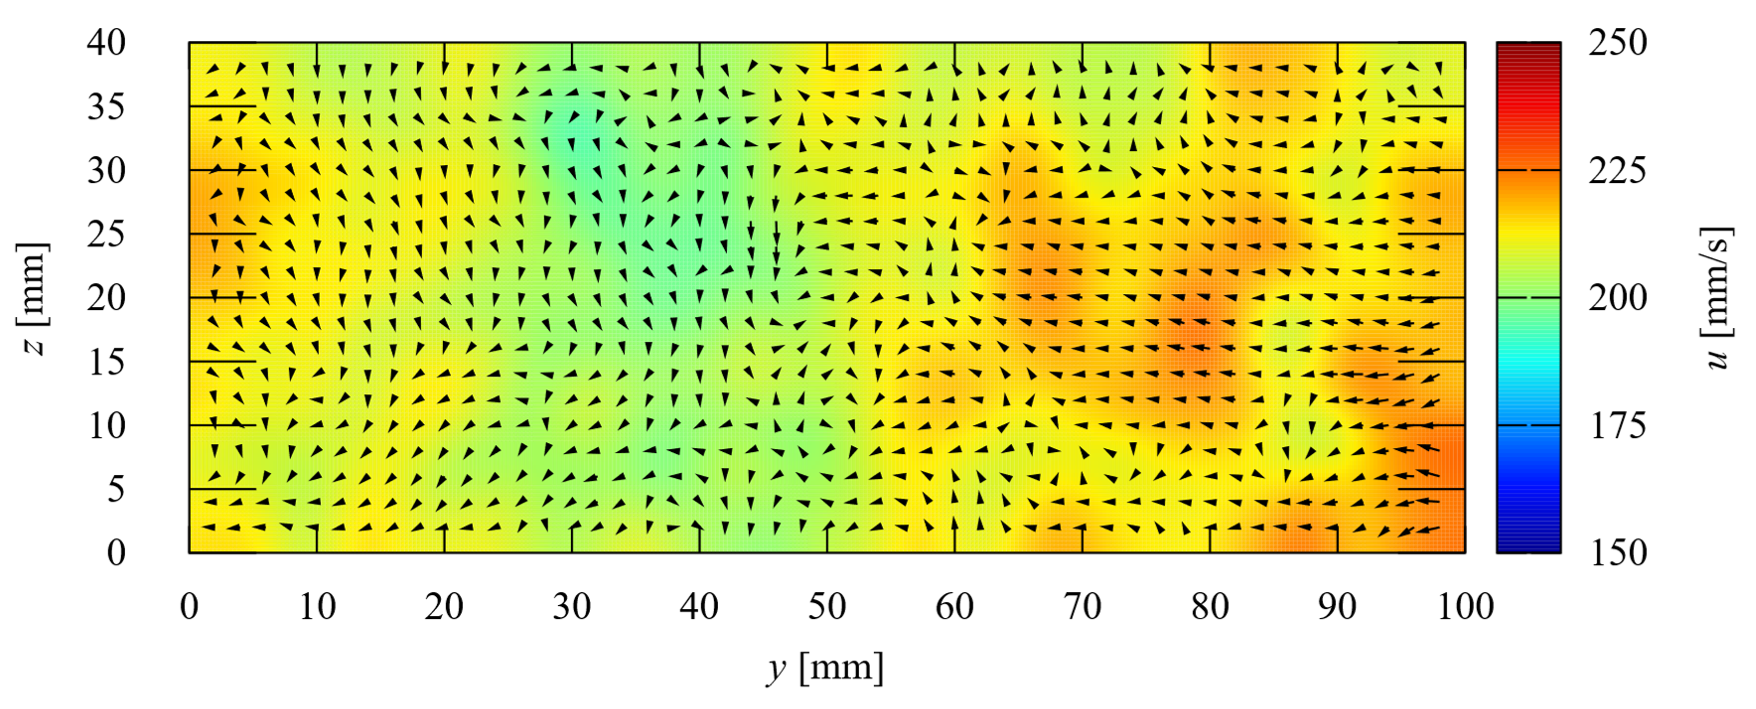
\includegraphics[keepaspectratio, width=82mm]{../images/uniform_velocity.png}
  \caption{Flow velocity : Uniform}
  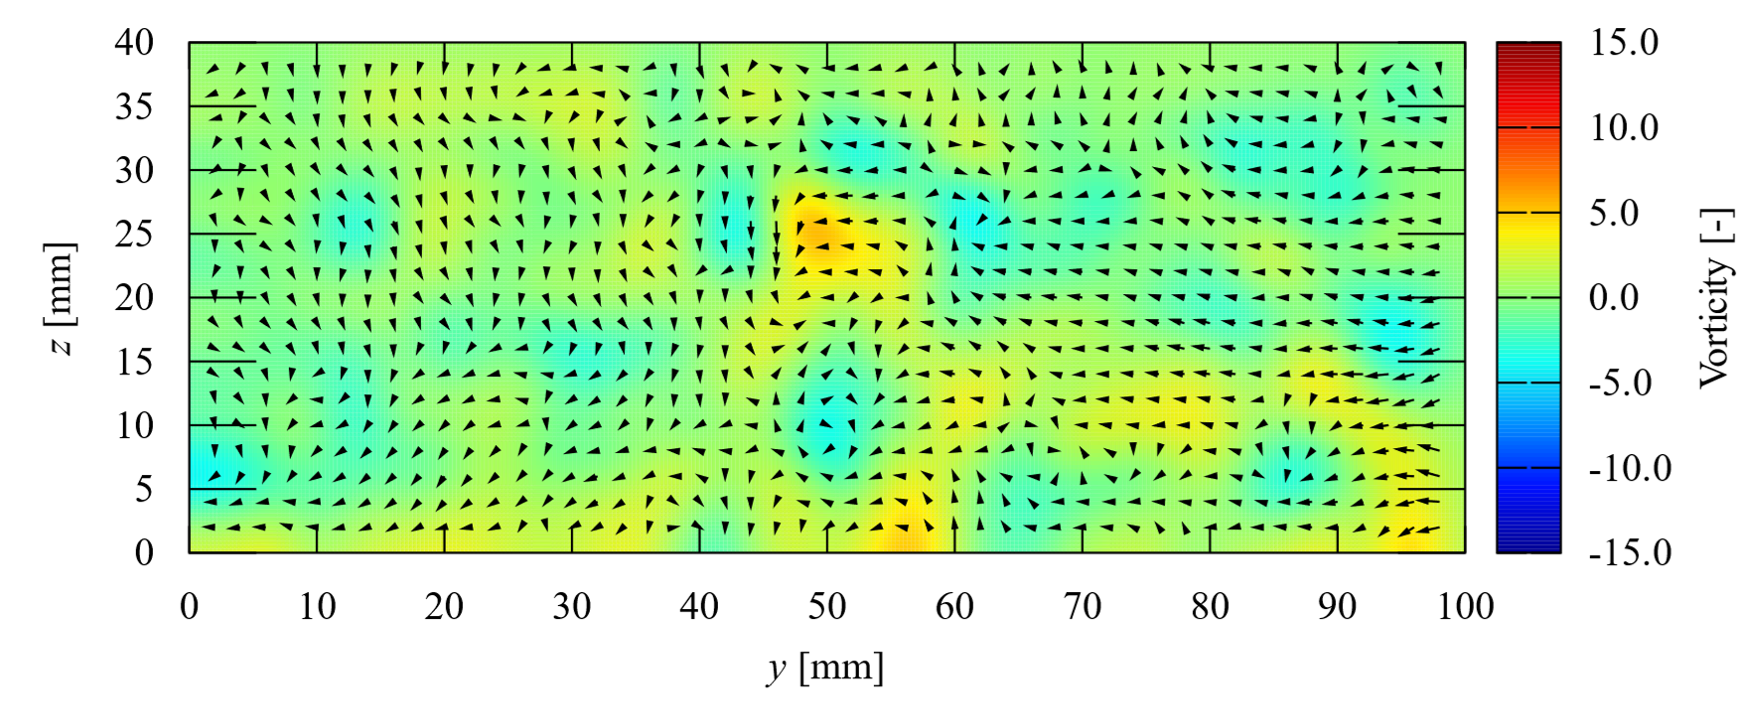
\includegraphics[keepaspectratio, width=82mm]{../images/uniform_vorticity.png}
  \caption{Vorticity : Uniform}
\end{figure}

\section{マッチングアルゴリズムの検討}
\subsection{最小二乗法によるクラスタ直線の取得}
速度ベクトルを得るために,クラスタどうしのマッチングを行う.
今回は,最小二乗法を用いてクラスタの持つ直線を取得し,
その係数を用いてマッチングを行った.

\begin{eqnarray*}
  i &:& \text{クラスタ番号}\\
  j &:& \text{フレーム番号}
\end{eqnarray*}

\subsubsection*{$\blacksquare$ 最小二乗法}
最小二乗法による三次元直線の式は以下のようになる.
今回は$n$を基準として,$y$と$z$を求めた.
\begin{eqnarray*}
  y_i &=& a_{1i}n_i + b_{1i}\\
  z_i &=& a_{2i}n_i + b_{2i}
\end{eqnarray*}

\subsubsection*{$\blacksquare$ 係数の計算}
また,係数の計算は以下のようになる.
ここで,$N_i$は$i$番目のクラスタの持つ粒子数,
$n_{ij}$は$j$番目の粒子のフレーム数,
$y_{ij}$は$j$番目の粒子の$y$方向の位置である.
\begin{eqnarray*}
  a_{1i} &=& \frac{N_i \sum_{j=1}^{N_i} n_{ij} y_{ij} - \sum_{j=1}^{N_i} n_{ij} \sum_{j=1}^{N_i} y_{ij}}{N_i \sum_{j=1}^{N_i} n_{ij}^2 - (\sum_{j=1}^{N_i} n_{ij})^2}\\
  b_{1i} &=& \frac{\sum_{j=1}^{N_i} y_{ij} - a_{1i} \sum_{j=1}^{N} n_{ij}}{N_i}\\
\end{eqnarray*}
※ $n-y$平面についてのみ記述,$n-z$平面も同様\\

\subsection{マッチングアルゴリズム}
\subsubsection*{(1) コサイン類似度}
コサイン類似度を以下の式を用いて計算し,直線の傾きを比較する.
\begin{eqnarray*}
  \vec{v_{ai} }&=& (a_{1i}, a_{2i})\\
  \vec{v_{ai'}} &=& (a_{1i'}, a_{2i'})\\
  \cos \theta &=& \frac{v_i \cdot v_i'}{|v_i||v_i'|}
\end{eqnarray*}

\subsubsection*{(2) ユークリッド距離}
\subsubsection*{$\blacksquare$ クラスタの位置}
クラスタの位置は平均値を用いる.\\
\begin{eqnarray*}
  y'_i = \frac{1}{N_i} \sum_{j=1}^{N} y_{ij} &:& y方向位置  \\
  z'_i = \frac{1}{N_i} \sum_{j=1}^{N} z_{ij} &:& z方向位置  \\
  n'_i = \frac{1}{N_i} \sum_{j=1}^{N} n_{ij} &:& フレーム数 \\
\end{eqnarray*}

\subsubsection*{$\blacksquare$ ユークリッド距離}
次に,ユークリッド距離を以下の式を用いて計算し,直線の位置を計算する.
\begin{eqnarray*}
  \vec{v_i} &=& (n_i, y_i, z_i)\\
  \vec{v_{i'}} &=& (n_{i'}, y_{i'}, z_{i'})\\
  d_{ny} &=& \sqrt{(n_i - n_{i'})^2 + (y_i - y_{i'})^2}\\
  d_{nz} &=& \sqrt{(n_i - n_{i'})^2 + (z_i - z_{i'})^2}\\
  d_{yz} &=& \sqrt{(y_i - y_{i'})^2 + (z_i - z_{i'})^2}
\end{eqnarray*}

\subsubsection*{$\blacksquare$ マッチング}
粒子のマッチングは,
上記で計算してきたコサイン類似度とユークリッド距離に重み係数をかけ合わせ,以下の式で計算する.
\begin{eqnarray*}
  D &=& C_1 \times (1- cos\theta) + C_2\times d_{ny} + C_3 \times d_{nz} + C_4 \times d_{yz}\\
  C_i &:& 重み係数 (合計が1になるように設定)\\
\end{eqnarray*}

\section{来週の予定}
\begin{itemize}
  \item マッチングアルゴリズムの検討 (続き)
\end{itemize}

\end{document}